%%%%%%%%%%%%%%%%%%%%%%%%%%%%%%%%%%%%%%%%%%%%%%%%%%%%%%%%%%%%%%%%%%%%%%%%
%                                                                      %
%     File: Thesis_Simulation.tex                                      %
%     Tex Master: Thesis.tex                                           %
%                                                                      %
%     Author: Andre C. Marta                                           %
%     Last modified :  05 Aug 2026                                     %
%                                                                      %
%%%%%%%%%%%%%%%%%%%%%%%%%%%%%%%%%%%%%%%%%%%%%%%%%%%%%%%%%%%%%%%%%%%%%%%%

\chapter{Implementation}
\label{chapter:implementation}

This chapter describes the software stack, nodes, and co-simulation setups used to implement and test the cooperative tethered control system. It details the code generation pipeline, the modular C++ ROS 2 package architecture, the cooperative mission state machine, and the integration of the MoorDyn physics engine and virtual winch controller within the Gazebo simulation environment.

\section{Software Environment and Code Generation}
\label{sec:sim_software_stack}

The software architecture is implemented on top of the Linux Ubuntu 22.04 LTS operating system using the \gls{ros} 2 (Robot Operating System) Humble Hawksbill middleware. For the design and generation of the optimization solvers of the \gls{nmpc} controllers, a symbolic code generation pipeline is employed. 

The code generation pipeline consists of the following components:
\begin{itemize}
    \item \textbf{CasADi Symbolic Framework:} A Python script is written for each vehicle (UAV and USV) to define the state, control, and parameter variables symbolically. CasADi handles the automatic differentiation, compiling the non-linear dynamics equations and evaluating analytical Jacobians and Hessian approximations.
    \item \textbf{Acados Template Library:} Consumes the CasADi symbolic models to generate highly optimized, native C code solvers. Acados bypasses generic optimization libraries by generating customized solvers tailored to the specific OCP structure.
    \item \textbf{High-Performance Kernels:} The exported C code is compiled utilizing the BLASFEO (Basic Linear Algebra Subprograms for Embedded Optimization) library, which optimizes processor cache utilization for small-to-medium-sized matrices. The linearized QP subproblems are solved using HPIPM (High-Performance Interior-Point Method), which implements a structured primal-dual interior-point method.
\end{itemize}

The temporal configuration of the NMPC solvers is configured independently for the two platforms to balance physical response rates and solver execution times:
\begin{itemize}
    \item \textbf{UAV Solver:} Discretized with a control period of $T_{s,UAV} = 0.02\,\text{s}$ ($50\,\text{Hz}$) and a prediction horizon of $N_{UAV} = 50$ intervals, yielding a total prediction horizon of $T_{f,UAV} = 1.0\,\text{s}$.
    \item \textbf{USV Solver:} Discretized with a control period of $T_{s,USV} = 0.1\,\text{s}$ ($10\,\text{Hz}$) and a prediction horizon of $N_{USV} = 20$ intervals, yielding a total prediction horizon of $T_{f,USV} = 2.0\,\text{s}$.
\end{itemize}

\section{ROS 2 Software Architecture}
\label{sec:sim_ros_architecture}

The system software is organized into modular ROS 2 packages, ensuring decoupling between control, estimation, simulation, and mission coordination.

\subsection{Workspace Structure and Package Modularity}
The ROS 2 workspace is organized into five primary packages, summarized in Table~\ref{tab:ros_packages}.

\begin{table}[H]
\centering
\caption{Summary of the modular ROS 2 packages in the cooperative workspace.}
\begin{tabular}{llp{7.5cm}}
\toprule
Package Name & Language & Primary Responsibility \\
\midrule
\texttt{bringup} & Python/YAML & System launch files, configuration files, and coordinate frame parameters. \\
\texttt{uav\_mpc} & C++/Python & UAV Acados solver generation, telemetry mapping, and position NMPC. \\
\texttt{usv\_mpc} & C++/Python & USV Acados solver generation, thruster allocation mapping, and tracking NMPC. \\
\texttt{moordyn\_tether} & C++ & MoorDyn mooring line node wrapper and active winch controller. \\
\texttt{ats\_mission} & C++ & Mission coordinator managing takeoff, orbiting, landing, and FSM transitions. \\
\bottomrule
\end{tabular}
\label{tab:ros_packages}
\end{table}

\subsection{Code Design Pattern: Library and ROS Wrapper}
To ensure code standard compliance, portability, and readability, all control nodes are implemented using a strict three-layer design pattern:
\begin{enumerate}
    \item \textbf{The Entry Point (\texttt{\_main.cpp}):} A minimal file containing only the main initialization function, instantiating the node wrapper, and spinning the ROS 2 executor.
    \item \textbf{The ROS Wrapper (\texttt{\_node.cpp/hpp}):} Handles all ROS-related tasks. It loads configuration parameters from YAML files, initializes publishers and subscribers, sets up timers, and manages the publishing of tf2 coordinate frame transformations. No mathematical calculations or control-oriented logic are written in this layer.
    \item \textbf{The Logic Pipeline (\texttt{\_pipeline.cpp/hpp}):} A pure C++ class that is completely independent of ROS. It uses native C++ and Eigen library types to execute the calculations. It wraps the Acados C structure, updates the states and parameters, runs the optimization solver, and maps virtual forces to actuator commands.
\end{enumerate}

To support multi-robot simulation and prevent topic collisions, all topic subscriptions and publications inside the nodes are written using relative topic names. This allows namespaces (e.g., \texttt{/wamv1/odom} and \texttt{/wamv2/odom}) to isolate vehicle telemetry.

\subsection{Cooperative Mission Finite State Machine}
The coordination of the cooperative UAV-USV mission is managed by the \texttt{mission\_manager} node inside the \texttt{ats\_mission} package. The coordinator implements a Finite State Machine (FSM) to orchestrate the flight phases of the drone relative to the ship, as illustrated in Figure~\ref{fig:mission_fsm}:
\begin{itemize}
    \item \textbf{IDLE:} Initial state. Nodes check sensor telemetry, establish the tether connection frames, and wait for the start command.
    \item \textbf{TAKEOFF:} Triggers autonomous UAV takeoff. The quadrotor rises vertically to a safe hovering altitude directly above the WAM-V helideck ($z_a = 3.0\,\text{m}$ relative to the deck). The USV and winch remain stationary.
    \item \textbf{COOPERATIVE\_TRACKING:} The active phase. The USV starts tracking its planar trajectory, and the UAV starts its orbit tracking or path-following sequence centered on the USV anchor. The winch is activated in either geometric or tension-regulated spooling mode to manage tether slack.
    \item \textbf{LANDING:} Triggered at the end of the mission. The USV reduces speed or hovers. The UAV approaches the catamaran deck, while the winch actively spools in the tether, tensioning the line to guide the quadrotor safely onto the deck.
\end{itemize}

\begin{figure}[H]
    \centering
    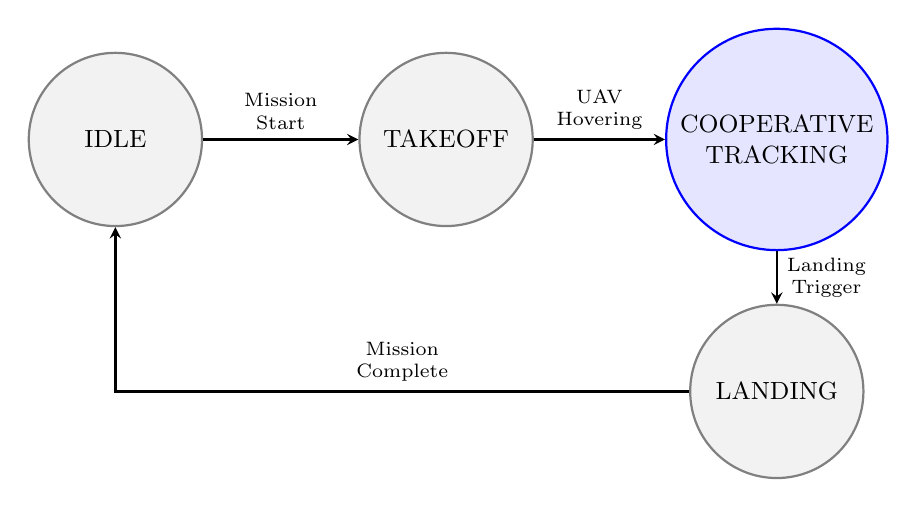
\begin{tikzpicture}[
        state/.style={draw, circle, minimum size=2.2cm, align=center, fill=gray!10, draw=gray, thick, font=\small},
        active_state/.style={draw, circle, minimum size=2.2cm, align=center, fill=blue!10, draw=blue, thick, font=\small},
        >=stealth,
        thick,
        node distance=4.2cm
    ]
        \node[state] (idle) {IDLE};
        \node[state, right of=idle] (takeoff) {TAKEOFF};
        \node[active_state, right of=takeoff] (tracking) {COOPERATIVE\\TRACKING};
        \node[state, below of=tracking, node distance=3.2cm] (landing) {LANDING};
        
        \draw[->] (idle) -- node[above, font=\scriptsize, align=center] {Mission\\Start} (takeoff);
        \draw[->] (takeoff) -- node[above, font=\scriptsize, align=center] {UAV\\Hovering} (tracking);
        \draw[->] (tracking) -- node[right, font=\scriptsize, align=center] {Landing\\Trigger} (landing);
        \draw[->] (landing) -| node[above, pos=0.25, font=\scriptsize, align=center] {Mission\\Complete} (idle);
    \end{tikzpicture}
    \caption{Finite State Machine (FSM) state transition diagram for the cooperative mission coordinator.}
    \label{fig:mission_fsm}
\end{figure}

\section{Co-Simulation Setup in Gazebo Harmonic}
\label{sec:sim_gazebo_setup}

The co-simulation environment is built in Gazebo Harmonic, which handles the multi-body physics, collisions, and environmental perturbations. The software stack integrates the simulator with the control pipeline through communication bridges:
\begin{itemize}
    \item \textbf{PX4 SITL and micro XRCE-DDS Bridge:} The x500 quadrotor simulation runs the actual PX4 Autopilot flight firmware in a Software-in-the-Loop (SITL) wrapper. The micro XRCE-DDS bridge manages the high-rate, low-latency exchanges between the PX4 middleware and the ROS 2 network, allowing the subscription to high-frequency state estimation (odometry, vehicle local position) and the publishing of offboard attitude rate and thrust targets.
    \item \textbf{ROS-Gazebo Bridge:} Maps the simulation clock, joint state commands (steerable thruster angles, propeller speeds), and winch actuator commands from ROS 2 to the Gazebo physics engine.
    \item \textbf{Time Synchronization:} To prevent time drift between the simulator and the controller nodes, all ROS 2 nodes are configured to run using simulation time. The Gazebo simulator publishes the simulation clock on the \texttt{/clock} topic, which is used by the ROS 2 executor to synchronize node timers.
\end{itemize}

\section{MoorDyn and Winch Integration}
\label{sec:sim_moordyn_integration}

The physical coupling forces and winch spooling rates are simulated through the integration of the MoorDyn mooring line library in the ROS 2 node \texttt{moordyn\_tether\_node}.

The integration is structured as follows:
\begin{itemize}
    \item \textbf{Coordinate Frame Tracking:} The C++ node tracks the relative transformation between the USV deck anchor point and the UAV center of gravity utilizing the \texttt{tf2} listener. 
    \item \textbf{Boundary Node Updates:} At a frequency of $100\,\text{Hz}$, the node updates the coordinates of the boundary nodes inside the MoorDyn solver with the tracked positions.
    \item \textbf{Winch Spooling Updates:} The node listens to winch spooling commands from the winch controller (\texttt{moordyn\_tether\_winch}) and updates the unstretched line length property inside the MoorDyn solver.
    \item \textbf{Force Propagation:} MoorDyn computes the internal segment tensions and propagates the resulting force vectors back to the boundary nodes, which are applied as external forces to the WAM-V and the x500 rigid bodies in Gazebo.
\end{itemize}
